% Brett
\chapter{Experience with Kokkos}
\section{Performance}
%Comparing Kokkos to Cuda and OpenMP
%Doing this for sanity check
%How we did this (used same algorithm and ran both, timed)
%some graphical results
%analysis of the results and differences
%conclusion that they are very similar performing
A feature that many programmers consider when deciding what the best solution is
to solve their problem, is performance. Since Kokkos uses Cuda and OpenMP as a
backend we thought that it was important to do some testing to ensure that
Kokkos performs as well as these two solutions. If Kokkos's performance was
worse then Cuda's or OpenMP's then programmers would use these other solutions
instead. The good news for Kokkos is that in our testing it performs almost
identically to Cuda and OpenMP. We did not spend an extensive amount of time
confirming our results. After a few pieces of supporting data we assumed that
the rest would give similar results because there is no information or evidence
that should give us reason to believe this trend will change. The rest of this
section will describe our strategy for testing performance of Kokkos versus Cuda
and Kokkos versus OpenMP, present graphs showing the differences observed,
analysis of these graphs, and then finally our concluding thoughts on the topic.
\\
\\
The general method that was used to create performance data for Kokkos, Cuda,
and OpenMP was to write algorithmically equivalent code for all three, make sure
that the layout of the data is the same, then time the runtime of each (one
after another). This process is pretty simple, but there is always noise in
timing. That is why we repeated the same exact calcuation five times and 
then use the average time. A couple things that should be noted include: we are
unsure how Kokkos does a reduction in the team_reduce() function, meaning we
could not write a Cuda reduction that we knew was algorithm equivalent and we
can not be sure that the compilers do the same optimizations. Although
we could have asked Dr. Carter Edwards (our liaison and one of the creators of 
Kokkos), the project's priorities had changed and it was decided to not pursue
this further. Regarding the second note, we tried to manually do some code
optimizations that compilers can handle in order to make sure the amount of work
each algorithm was the same (which is expected). Of course if one compiler has
more advanced optimization techniques that is a benefit that should not be
overlooked, but the goal of this testing was not to test performance against
ease of coding, but rather the overall performance differences of Kokkos to 
Cuda and Kokkos to OpenMP. \\
\\
Now we will look at some of the performance differences and similarities of
Kokkos, Cuda, and OpenMP. Here is a graph that shows the raw times of Kokkos
Cuda, Cuda, Kokkos OpenMP, and OpenMP:
$$\begin{figure}
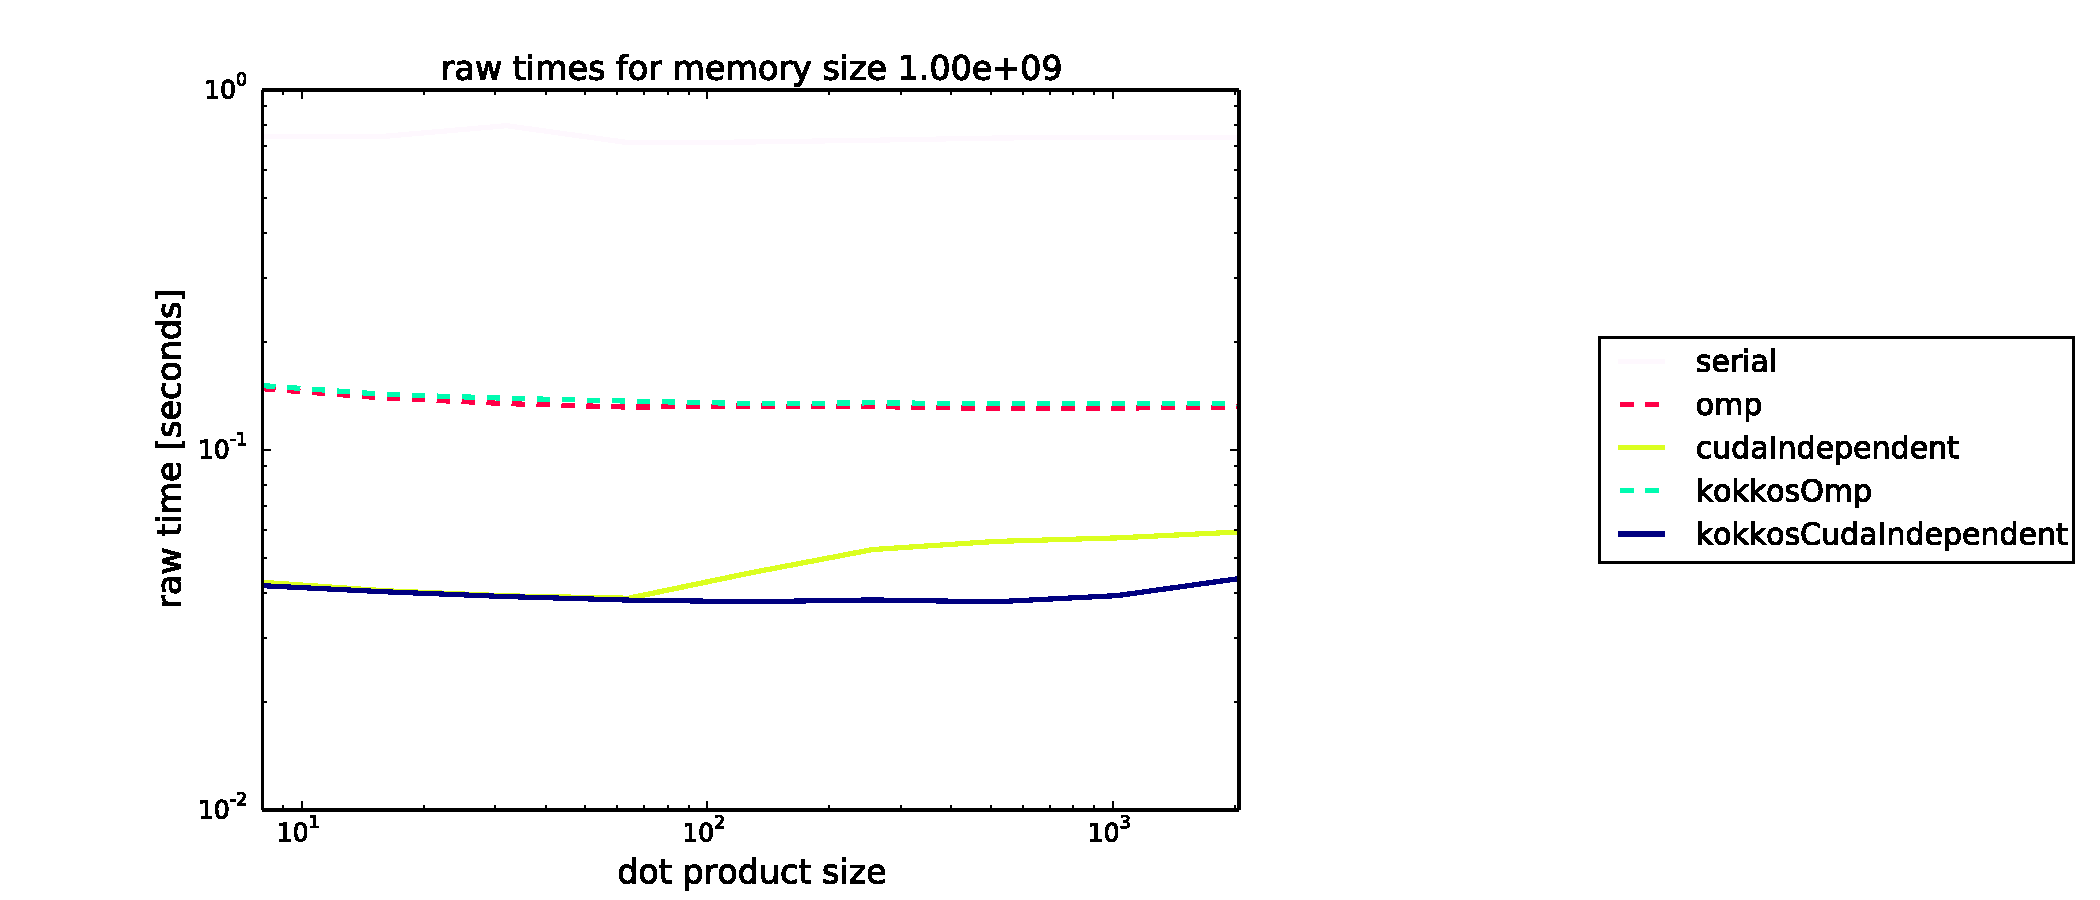
\includegraphics{CDDS_RawTimes_2d_largestSize_Comparison.pdf}
\caption{This graph plots the performance of Kokkos Cuda, Cuda, Kokkos OpenMP,
and OpenMP for ContractDataDataScalar with a memory size of 1 GB. 
The y-axis is time in
seconds, so closer to 0 is better. The x-axis plots different contraction sizes
in order to compare multiple points.}
\end{figure}$$
Notice how in this graph Kokkos OpenMP and OpenMP are almost perfectly
overlapping with Kokkos OpenMP. We are not quite sure why they are not perfectly
overlapping, but it appears that it is not random noise because it is pretty
consistent in this graph. However, the difference is so small it seems
insignificant. \\
\\
KokkosCuda versus Cuda, on the other hand, has some big differences. They are
identical for the smaller problems but diverge a significant amount for bigger
problems. One of the theories that we have as to why this trend exists is that
Kokkos may use a different block size than what we use in our Cuda algorithm.
We believe the reason this doesn't effect the smaller problem sizes is because
in both cases the maximum number of threads per block isn't being utilized, so
it does not make a difference, but clearly does in the bigger problem sizes.
$$\begin{figure}
\includegraphics{CFFS_RawTimes_2d_largestSize_Comparison.pdf}
\caption{This graph shows performance differences (or similarities in our case)
of the nested parallelism approach slicing.}
\end{figure}$$
In this graph it is clear that the Cuda slicing performance is almost identical
to the Kokkos slicing performance. This is important to show that both Kokkos's
and Cuda's use of shared memory results in the same performance. \\
\\
Overall, after seeing a handful of graphs that show Kokkos performs almost
identically to Cuda and to OpenMP, we accepted that Kokkos is not adding any
unneeded overhead. As stated before, there may be slight differences due to
compiler optimizations, but Kokkos seems to perform identically to the other
multithreading solutions.

\section{Snippets}
%Amount of work the programmer has to do is important
%control and complexity of code is important
%Much more complex than OpenMP, but follows a different paradigm
%Very similar to Cuda, except kernel is a functor
%Overall a pretty easy language, some magic values but pretty good
Another major factor that plays into whether or not a programmer uses a certain
language, feature, library, etcetera, is code complexity and ease of coding.
Although this can be subjective, there are a couple differences between the
language we would like to point out, especially regarding amount of code
required compared to Cuda or OpenMP (although comparing to OpenMP may be unfair)
and intuitiveness of the code (or readability). \\
\\
Regarding the amount of code required, comparing Kokkos to OpenMP does not seem
fair. Comparing OpenMP to almost anything seems unfair, because OpenMP requires
very little code and most of the work is done for you. Although OpenMP only
works on the CPU which is why it does not require the extra code that Kokkos
requires. In general, OpenMP cannot be compared to Kokkos. If the programmer
knows the code only needs to be multithreaded on the CPU and will never need
more threads then we would strongly advise them to use OpenMP because it is very
simple. However, that is not the niche that Kokkos is trying to fill. \\
\\
Kokkos compared to Cuda however, requires similar amounts of code and has a
close philosophy. Throughout the code comparison of Cuda and Kokkos we will show
code snippets and point out the differences and similarities directly. We will
start by showing the data setup, because the data needs to get onto the GPU
somehow, then we will move compare and contrast the Cuda kernel and the Kokkos
functor. 
\\
Here is code that shows the setup of the data on the GPU for Cuda:
$$\begin{figure}
\end{figure}$$
There are essentially thress steps in the process: declaring a pointer to the
data on the CPU, creating an array with the correct size on the GPU, then
copying the data over to the GPU from wherever the data is currently kept on the
CPU. This process is pretty simple and self-explanatory. Now let us compare that
to Kokkos:
$$\begin{figure}
\end{figure}$$
Our code starts with typedefs, although they are not required it is clear that
they are helpful because they are more compact 

\section{Bugs}

\section{Personal Experience and Thoughts}

